\chapter{Specifikacija programske potpore}

\section{Funkcionalni zahtjevi}

\noindent \textbf{Dionici:}

\begin{packed_enum}

	\item Neregistrirani korisnik
	\item Registrirani korisnik
	\begin{packed_enum}
		\item Građanin
		\item Službenik gradskog ureda
	\end{packed_enum}
	\item Administrator
	\item Razvojni tim
	\item Suradnici
	\begin{packed_enum}
		\item Nastavnik
		\item Demonstrator
	\end{packed_enum}

\end{packed_enum}

\noindent \textbf{Aktori i njihovi funkcionalni zahtjevi:}


\begin{packed_enum}
	\item  \underbar{Neregistrirani korisnik (inicijator) može:}

	\begin{packed_enum}

		\item podnositi anonimne prijave
		\item pratiti status prijave jedinstvenim brojem prijave
		\item imati uvid u postojeće prijave
		\item imati uvid u statistiku statusa prijava
		\item registrirati korisnički račun


	\end{packed_enum}

	\item  \underbar{Građanin (inicijator) može:}

	\begin{packed_enum}

		\item prijaviti se na korisnički račun
		\item odjaviti se s korisničkog računa
		\item pratiti status vlastitih prijava
		\item imati uvid u postojeće prijave
		\item imati uvid u statistiku statusa prijava
		\item izmijeniti podatke korisničkog računa

	\end{packed_enum}

	\item \underbar{Službenik gradskog ureda (inicijator) može:}

	\begin{packed_enum}

		\item obrađivati podnesene prijave
		\item objediniti nepovezane prijave po temi i lokaciji
		\item promijeniti status prijave
		\item pratiti i analizirati probleme u stvarnom vremenu
		\item izmijeniti podatke korisničkog računa

	\end{packed_enum}

	\item \underbar{Administrator (inicijator) može:}

	\begin{packed_enum}

		\item uređivati i brisati korisničke račune
		\item pristupiti bazi podataka
		\item kreirati i ukloniti gradski ured
		\item dodijeliti i ukloniti ulogu službenika gradskog ureda registriranom korisniku 
		\item dodijeliti i ukloniti ulogu administratora registriranom korisniku 
	\end{packed_enum}

	\item \underbar{Baza podataka (sudionik) može:}

	\begin{packed_enum}

		\item pohraniti sve podatke o korisnicima i njihovim ulogama
		\item pohraniti sve podatke o prijavljenim oštećenjima
		\item pohraniti sve podatke o kategorijama problema i gradskim uredima za njihovo obrađivanje

	\end{packed_enum}

\end{packed_enum}


\eject



\subsection{Obrasci uporabe}

\subsubsection{Opis obrazaca uporabe}

\noindent \underbar{\textbf{UC01 - Registracija korisničkog računa}}
\begin{packed_item}

	\item \textbf{Glavni sudionik: }Neregistrirani korisnik
	\item  \textbf{Cilj:} Stvaranje korisničkog račun za pristup sustavu
	\item  \textbf{Sudionici:} Baza podataka
	\item  \textbf{Preduvjet:} -
	\item  \textbf{Opis osnovnog tijeka:}

	\item[] \begin{packed_enum}

		\item Korisnik odabire opciju za prijavu
		\item Korisnik odabire opciju da nema korisnički račun
		\item Korisnik unosi potrebne podatke i potvrđuje unos
		\item Korisnik se upisuje u bazu podataka i korisnik se preusmjerava na početnu stranicu
	\end{packed_enum}

	\item  \textbf{Opis mogućih odstupanja:}

	\item[] \begin{packed_item}

		\item[3.a] Odabir već zauzetog korisničkog imena i/ili e-mail adrese, unos korisničkih podataka u neispravnom formatu, nepodudaranje lozinki
		\item[] \begin{packed_enum}

			\item Sustav obavještava korisnika o neuspjelom unosu i vraća ga na stranicu za registraciju
			\item Korisnik mijenja potrebne podatke te završava unos ili odustaje od registracije

		\end{packed_enum}
	\end{packed_item}
\end{packed_item}

\noindent \underbar{\textbf{UC02 - Prijava na korisnički račun}}
\begin{packed_item}

	\item \textbf{Glavni sudionik: }Registrirani korisnik
	\item  \textbf{Cilj:} Dobivanje pristupa korisničkom sučelju s ovlastima registriranog korisnika
	\item  \textbf{Sudionici:} Baza podataka
	\item  \textbf{Preduvjet:} Korisnik je obavio registraciju i njegovi podaci se nalaze u bazi podataka
	\item  \textbf{Opis osnovnog tijeka:}

	\item[] \begin{packed_enum}

		\item Korisnik odabire opciju za prijavu
		\item Korisnik unosi korisničko ime i lozinku te potvrđuje unos
		\item Korisnik se preusmjerava na početnu stranicu
	\end{packed_enum}

	\item  \textbf{Opis mogućih odstupanja:}

	\item[] \begin{packed_item}

		\item[2.a] Neispravni unos korisničkog imena i/ili lozinke
		\item[] \begin{packed_enum}

			\item Sustav obavještava korisnika o neuspjelom unosu i vraća ga na stranicu za prijavu
			\item Korisnik unosi ispravne podatke te završava unos ili odustaje od prijave

		\end{packed_enum}
	\end{packed_item}
\end{packed_item}

\noindent \underbar{\textbf{UC03 - Odjava s korisničkog računa}}
\begin{packed_item}

	\item \textbf{Glavni sudionik: }Registrirani korisnik
	\item  \textbf{Cilj:} Izlazak iz korisničkog sučelja
	\item  \textbf{Sudionici:} Baza podataka
	\item  \textbf{Preduvjet:} Korisnik je obavio prijavu na korisnički račun
	\item  \textbf{Opis osnovnog tijeka:}

	\item[] \begin{packed_enum}

		\item Korisnik odabire opciju za odjavu
		\item Korisnik se preusmjerava na početnu stranicu
	\end{packed_enum}
\end{packed_item}


\noindent \underbar{\textbf{UC04 - Kreiranje gradskog ureda}}
\begin{packed_item}

	\item \textbf{Glavni sudionik: }Administratori
	\item  \textbf{Cilj:} Kreiranje gradskog ureda
	\item  \textbf{Sudionici:} Baza podataka
	\item  \textbf{Preduvjet:} Korisnik je prijavljen i ima administrator ovlasti
	\item  \textbf{Opis osnovnog tijeka:}

	\item[] \begin{packed_enum}

		\item Korisnik otvara padajući izbornik
		\item Korisnik odabire opciju za kreiranje gradskog ureda
		\item Korisnik unosi potrebne podatke i potvrđuje unos
		\item Gradski ured se upisuje u bazu podataka i korisnik se preusmjerava na početnu stranicu

	\end{packed_enum}

	\item  \textbf{Opis mogućih odstupanja:}

	\item[] \begin{packed_item}

		\item[3.a] Odabir već zauzetog imena gradskog ureda
		\item[] \begin{packed_enum}

			\item Sustav obavještava korisnika o neuspjelom unosu i vraća ga na stranicu za kreiranje gradskog ureda
			\item Korisnik mijenja potrebne podatke te završava unos ili odustaje od kreiranja gradskog ureda

		\end{packed_enum}
		\item[3.b] Nije odabrana nijedna kategorija oštećenja kojom će gradski ured upravljati
		\item[] \begin{packed_enum}

			\item Sustav obavještava korisnika o obveznom unosu barem jedne kategorije oštećenja kojom će ured upravljati
			\item Korisnik odabire barem jednu kategoriju oštećenja te završava unos ili odustaje od kreiranja gradskog ureda

		\end{packed_enum}

	\end{packed_item}
\end{packed_item}


\noindent \underbar{\textbf{UC05 - Uklanjanje gradskog ureda}}
\begin{packed_item}

	\item \textbf{Glavni sudionik: }Administrator
	\item  \textbf{Cilj:} Uklanjanje gradskog ureda
	\item  \textbf{Sudionici:} Baza podataka
	\item  \textbf{Preduvjet:} Korisnik je prijavljen i ima administrator ovlasti, gradski ured postoji
	\item  \textbf{Opis osnovnog tijeka:}

	\item[] \begin{packed_enum}

		\item Korisnik otvara padajući izbornik
		\item Korisnik odabire opciju za pregled gradskih ureda
		\item Korisnik odabire gradski ured
		\item Korisnik odabire opciju za uklanjanje gradskog ureda 
		\item Gradski ured se uklanja iz baze podataka i korisnik se preusmjerava na stranicu za pregled gradskih ureda
	\end{packed_enum}
\end{packed_item}


\noindent \underbar{\textbf{UC06 - Dodjela uloge službenika gradskog ureda}}
\begin{packed_item}

	\item \textbf{Glavni sudionik: }Administrator
	\item  \textbf{Cilj:} Dodjeljivanje uloge službenika gradskog ureda registriranom korisniku
	\item  \textbf{Sudionici:} Baza podataka
	\item  \textbf{Preduvjet:} Korisnik je prijavljen i ima administratorske ovlasti, postoji odgovarajući gradski ured za registriranog korisnika
	\item  \textbf{Opis osnovnog tijeka:}

	\item[] \begin{packed_enum}

		\item Korisnik otvara padajući izbornik 
		\item Korisnik odabire opciju za pregled popisa korisničkih računa
		\item Korisnik odabire korisnički račun
		\item Korisnik odabire opciju za dodjelu uloge službenika gradskog ureda
		\item Registrirani korisnik dobiva ulogu službenika gradskog ureda i korisnik se preusmjerava na pregled korisničkog računa
	\end{packed_enum}
\end{packed_item}


\noindent \underbar{\textbf{UC07 - Pregled korisničkog računa}}
\begin{packed_item}

	\item \textbf{Glavni sudionik: }Registrirani korisnik
	\item  \textbf{Cilj:} Pregledavanje korisničkog račun
	\item  \textbf{Sudionici:} Baza podataka
	\item  \textbf{Preduvjet:} Korisnik je obavio prijavu na korisnički račun
	\item  \textbf{Opis osnovnog tijeka:}

	\item[] \begin{packed_enum}

		\item Korisnik otvara padajući izbornik
		\item Korisnik odabire opciju za pregled vlastitog korisničkog računa
	\end{packed_enum}
\end{packed_item}


\noindent \underbar{\textbf{UC08 - Uređivanje podataka korisničkog računa}}
\begin{packed_item}

	\item \textbf{Glavni sudionik: }Registrirani korisnik
	\item  \textbf{Cilj:} Promjena podataka na vlastitom korisničkom računu 
	\item  \textbf{Sudionici:} Baza podataka
	\item  \textbf{Preduvjet:} Korisnik je obavio prijavu na korisnički račun
	\item  \textbf{Opis osnovnog tijeka:}

	\item[] \begin{packed_enum}

		\item Korisnik otvara padajući izbornik
		\item Korisnik odabire opciju za pregled vlastitog korisničkog računa
		\item Korisnik odabire opciju za uređivanje korisničkih podataka
		\item Korisnik uređuje korisničke podatke i potvrđuje promjene
		\item Korisnički podaci se ažuriraju u bazi podataka i korisnik se preusmjerava na pregled vlastitog korisničkog računa
	\end{packed_enum}

	\item  \textbf{Opis mogućih odstupanja:}

	\item[] \begin{packed_item}

		\item[4.a] Odabir već zauzetog korisničkog imena i/ili e-mail adrese, unos korisničkog podatka u neispravnom formatu, nepodudaranje lozinki
		\item[] \begin{packed_enum}

			\item Sustav obavještava korisnika o neuspjelom unosu i vraća ga na uređivanje korisničkih podataka
			\item Korisnik mijenja potrebne podatke te završava unos ili odustaje od uređivanja korisničkih podataka

		\end{packed_enum}
	\end{packed_item}
\end{packed_item}


\noindent \underbar{\textbf{UC09 - Brisanje korisničkog računa}}
\begin{packed_item}

	\item \textbf{Glavni sudionik: }Registrirani korisnik
	\item  \textbf{Cilj:} Uklanjanje vlastitog korisničkog računa
	\item  \textbf{Sudionici:} Baza podataka
	\item  \textbf{Preduvjet:} Korisnik je obavio prijavu na korisnički račun
	\item  \textbf{Opis osnovnog tijeka:}

	\item[] \begin{packed_enum}

		\item Korisnik otvara padajući izbornik
		\item Korisnik odabire opciju za pregled vlastitog korisničkog računa
		\item Korisnik odabire opciju za brisanje korisničkog računa
		\item Korisnik povrđuje odluku i korisnik se preusmjerava na početnu stranicu
	\end{packed_enum}
\end{packed_item}


\noindent \underbar{\textbf{UC10 - Kreiranje anonimne prijave oštećenja}}
\begin{packed_item}

	\item \textbf{Glavni sudionik: }Neregistrirani korisnik
	\item  \textbf{Cilj:} Prijava oštećenja
	\item  \textbf{Sudionici:} Baza podataka
	\item  \textbf{Preduvjet:} -
	\item  \textbf{Opis osnovnog tijeka:}

	\item[] \begin{packed_enum}

		\item Korisnik odabire opciju za prijavu oštećenja
		\item Korisnik unosi potrebne podatke i potvrđuje unos
		\item Prijava oštećenja se upisuje u bazu podataka i korisnik dobiva jedinstveni broj prijave
	\end{packed_enum}

	\item  \textbf{Opis mogućih odstupanja:}

	\item[] \begin{packed_item}

		\item[2.a] Neuneseni obvezni podaci i/ili podaci uneseni u neispravnom formatu 
		\item[] \begin{packed_enum}

			\item Sustav obavještava korisnika o neuspjelom unosu i vraća ga na stranicu za prijavu oštećenja
			\item Korisnik mijenja potrebne podatke te završava unos ili odustaje od prijave oštećenja

		\end{packed_enum}
	\end{packed_item}
\end{packed_item}


\noindent \underbar{\textbf{UC11 - Kreiranje prijave oštećenja}}
\begin{packed_item}

	\item \textbf{Glavni sudionik: }Registrirani korisnik
	\item  \textbf{Cilj:} Prijava oštećenja
	\item  \textbf{Sudionici:} Baza podataka
	\item  \textbf{Preduvjet:} Korisnik je prijavljen
	\item  \textbf{Opis osnovnog tijeka:}

	\item[] \begin{packed_enum}

		\item Korisnik odabire opciju za prijavu oštećenja
		\item Korisnik unosi potrebne podatke i potvrđuje unos
		\item Prijava oštećenja se upisuje u bazu podataka i korisnik se preusmjerava na početnu stranicu
	\end{packed_enum}

	\item  \textbf{Opis mogućih odstupanja:}

	\item[] \begin{packed_item}

		\item[2.a] Neuneseni obvezni podaci i/ili podaci uneseni u neispravnom formatu 
		\item[] \begin{packed_enum}

			\item Sustav obavještava korisnika o neuspjelom unosu i vraća ga na stranicu za prijavu oštećenja
			\item Korisnik mijenja potrebne podatke te završava unos ili odustaje od prijave oštećenja

		\end{packed_enum}
	\end{packed_item}
\end{packed_item}


\noindent \underbar{\textbf{UC12 - Provjera statusa anonimne prijave oštećenja}}
\begin{packed_item}

	\item \textbf{Glavni sudionik: } Neregistrirani korisnik
	\item  \textbf{Cilj:} Provjera statusa anonimne prijave oštećenja
	\item  \textbf{Sudionici:} Baza podataka
	\item  \textbf{Preduvjet:} Podnesena prijava oštećenja
	\item  \textbf{Opis osnovnog tijeka:}

	\item[] \begin{packed_enum}

		\item Korisnik odabire opciju za provjeru statusa prijave oštećenja
		\item Korisnik unosi jedinstveni broj prijave i potvrđuje unos
	\end{packed_enum}

	\item  \textbf{Opis mogućih odstupanja:}

	\item[] \begin{packed_item}

		\item[2.a] Jedinstveni broj prijave ne postoji ili je unesen u neispravnom formatu
		\item[] \begin{packed_enum}

			\item Sustav obavještava korisnika o neuspjelom unosu i vraća ga na stranicu za provjeru statusa prijave oštećenja
			\item Korisnik unosi ispravni jedinstveni broj prijave i završava unos ili odustaje od provjere statusa prijave oštećenja

		\end{packed_enum}

	\end{packed_item}
\end{packed_item}


\noindent \underbar{\textbf{UC13 - Provjera statusa prijave oštećenja}}
\begin{packed_item}

	\item \textbf{Glavni sudionik: } Registrirani korisnik
	\item  \textbf{Cilj:} Provjera statusa vlastite prijave oštećenja
	\item  \textbf{Sudionici:} Baza podataka
	\item  \textbf{Preduvjet:} Podnesena prijava oštećenja, korisnik je prijavljen
	\item  \textbf{Opis osnovnog tijeka:}

	\item[] \begin{packed_enum}

		\item Korisnik odabire opciju za provjeru statusa prijave oštećenja
		\item Korisnik odabire prijavu oštećenja za koju želi provjeriti status oštećenja
	\end{packed_enum}
\end{packed_item}


\noindent \underbar{\textbf{UC14 - Pregled prijave oštećenja}}
\begin{packed_item}

	\item \textbf{Glavni sudionici: } Registrirani korisnik, Neregistrirani korisnik
	\item  \textbf{Cilj:} Pregled prijave oštećenja
	\item  \textbf{Sudionici:} Baza podataka
	\item  \textbf{Preduvjet:} -
	\item  \textbf{Opis osnovnog tijeka:}

	\item[] \begin{packed_enum}

		\item Pregled prijave oštećenja
		\item Korisniku se otvara pregled prijavljeno oštećenje 
	\end{packed_enum}
\end{packed_item}


\noindent \underbar{\textbf{UC15 - Promjena statusa prijave oštećenja}}
\begin{packed_item}

	\item \textbf{Glavni sudionik: }Službenik gradskog ureda
	\item  \textbf{Cilj:} Promjena statusa prijave oštećenja
	\item  \textbf{Sudionici:} Baza podataka
	\item  \textbf{Preduvjet:} Podnesena prijava oštećenja, korisnik ima ulogu službenika gradskog ureda
	\item  \textbf{Opis osnovnog tijeka:}

	\item[] \begin{packed_enum}

		\item Korisnik odabire opciju za prikaz popisa prijavljenih oštećenja
		\item Korisnik odabire prijavu oštećenja
		\item Korisnik odabire opciju za promjenu statusa prijave i potvrđuje promjenu
		\item Status prijave oštećenja se ažurira u bazi podataka i korisnik se preusmjerava na pregled prijave oštećenja
	\end{packed_enum}
\end{packed_item}


\noindent \underbar{\textbf{UC16 - Provjera statistike statusa prijave oštećenja}}
\begin{packed_item}

	\item \textbf{Glavni sudionici: } Neregistrirani korisnik, Registrirani korisnik
	\item  \textbf{Cilj:} Provjera statistike statusa prijave oštećenja
	\item  \textbf{Sudionici:} Baza podataka
	\item  \textbf{Preduvjet:} -
	\item  \textbf{Opis osnovnog tijeka:}

	\item[] \begin{packed_enum}

		\item Korisnik odabire opciju za provjeru statistike statusa prijava oštećenja
		\item Korisniku se otvara pregled statistike statusa prijava oštećenja
	\end{packed_enum}
\end{packed_item}


\noindent \underbar{\textbf{UC17 - Objedinjavanje nepovezanih prijava oštećenja}}
\begin{packed_item}

	\item \textbf{Glavni sudionik: } Službenik gradskog ureda
	\item  \textbf{Cilj:} Objediniti nepovezane prijave oštećenja po temi i lokaciji
	\item  \textbf{Sudionici:} Baza podataka
	\item  \textbf{Preduvjet:} Postoje prijave oštećenja s istom temom i lokacijom, korisnik ima ulogu službenika gradskog ureda
	\item  \textbf{Opis osnovnog tijeka:}

	\item[] \begin{packed_enum}

		\item Korisnik odabire opciju za prikaz popisa prijavljenih oštećenja
		\item Korisnik odabire opciju za objedinjavanje prijava oštećenja
		\item Korisnik odabire dvije ili više prijava oštećenja i potvrđuje odabir
		\item Prijave oštećenja se objedinjuju u bazi podataka i korisnik se preusmjerava na početnu stranicu
	\end{packed_enum}

	\item  \textbf{Opis mogućih odstupanja:}

	\item[] \begin{packed_item}

		\item[3.a] Korisnik je odabrao manje od dvije prijave oštećenja i pokušao napraviti objedinjavanje
		\item[] \begin{packed_enum}

			\item Sustav obavještava korisnika o neuspjelom pokušaju objedinjavanja i vraća ga na odabir prijava oštećenja
			\item Korisnik odabire više od dvije prijave oštećenja i potvrđuje odabir ili odustaje od objedinjavanja prijava oštećenja
		\end{packed_enum}

	\end{packed_item}
\end{packed_item}


\noindent \underbar{\textbf{UC18 - Dodjela kategorije za upravljanje gradskom uredu}}
\begin{packed_item}

	\item \textbf{Glavni sudionik: }Administrator
	\item  \textbf{Cilj:} Dodjela kategorije oštećenja kojom će određeni gradski ured upravljati
	\item  \textbf{Sudionici:} Baza podataka
	\item  \textbf{Preduvjet:} Gradski ured postoji, korisnik ima ulogu administratora
	\item  \textbf{Opis osnovnog tijeka:}

	\item[] \begin{packed_enum}

		\item Korisnik odabire padajući izbornik
		\item Korisnik odabire opciju pregleda gradskih ureda
		\item Korisnik odabire gradski ured
		\item Korisnik odabire opciju za dodavanje kategorija oštećenja 
		\item Korisnik radi odabir kategorija i potvđuje odabir
		\item Ažurirani popis kategorija oštećenja za koje je zadužen gradski ured se upisuje u bazu podataka i korisnik se preusmjerava na pregled profila gradskog ureda
	\end{packed_enum}

	\item  \textbf{Opis mogućih odstupanja:}

	\item[] \begin{packed_item}

		\item[4.a] Gradski ured već upravlja svim kategorijama oštećenja, ne postoji kategorija oštećenja kojom već ne upravlja neki gradski ured u istom mjestu
		\item[] \begin{packed_enum}

			\item Sustav obavještava korisnika da ne postoji kategorija oštećenja kojom gradski ured već ne upravlja ili da ne postoji kategorija kojom već ne upravlja neki gradski ured u istom mjestu
			\item Korisnik odustaje od dodjele kategorije za upravljanje gradskom uredu

		\end{packed_enum}
	\end{packed_item}
\end{packed_item}


\noindent \underbar{\textbf{UC19 - Uklanjanje kategorije za upravljanje iz gradskog ureda}}
\begin{packed_item}

	\item \textbf{Glavni sudionik: }Administrator
	\item  \textbf{Cilj:} Uklanjanje kategorije oštećenja kojom trenutno upravlja gradski ured
	\item  \textbf{Sudionici:} Baza podataka
	\item  \textbf{Preduvjet:} Gradski ured postoji, korisnik ima ulogu administratora
	\item  \textbf{Opis osnovnog tijeka:}

	\item[] \begin{packed_enum}

		\item Korisnik odabire padajući izbornik
		\item Korisnik odabire opciju pregleda gradskih ureda
		\item Korisnik odabire gradski ured
		\item Korisnik odabire opciju da uklanjanje kategorija oštećenja
		\item Korisnik radi odabir kategorija i potvđuje ga
		\item Ažurirani popis kategorija oštećenja za koje je zadužen gradski ured se upisuje u bazu podataka i korisnik se preusmjerava na pregled profila gradskog ureda
	\end{packed_enum}

	\item  \textbf{Opis mogućih odstupanja:}

	\item[] \begin{packed_item}

		\item[5.a] Korisnik je odabrao sve kategorije oštećenja 
		\item[] \begin{packed_enum}

			\item Sustav obavještava korisnika da je odabrao sve kategorije oštećenja i vraća ga na stranicu za uređivanje gradskog ureda s otvorenom opcijom odabira kategorija
			\item Korisnik odabire kategorije pazeći da ostavi barem jednu kategoriju i potvrđuje odabir ili odustaje od uklanjanja kategorija oštećenja kojima upravlja gradski ured

		\end{packed_enum}
	\end{packed_item}
\end{packed_item}


\noindent \underbar{\textbf{UC20 - Ponovno postavljanje zaboravljene lozinke}}
\begin{packed_item}

	\item \textbf{Glavni sudionik: }Registrirani korisnik
	\item  \textbf{Cilj:} Stvaranje nove lozinke za registriranog korisnika
	\item  \textbf{Sudionici:} Baza podataka
	\item  \textbf{Preduvjet:} Korisnik je registriran i njegovi podaci se nalaze u bazi podataka
	\item  \textbf{Opis osnovnog tijeka:}

	\item[] \begin{packed_enum}

		\item Korisnik odabire opciju za prijavu
		\item Korisnik odabire opciju za ponovno postavljanje zaboravljene lozinke
		\item Korisnik unosi e-mail adresu korisničkog računa i potvrđuje unos
		\item Korisnik dobiva personalizirani link na stranicu gdje mijenja lozinku
		\item Korisnik unosi novu lozinku i potvrđuje odabir
		\item Nova lozinka sprema se u bazu podataka i korisnik se preusmjerava na početnu stranicu
	\end{packed_enum}

	\item  \textbf{Opis mogućih odstupanja:}

	\item[] \begin{packed_item}

		\item[3.a] Unesena e-mail adresa ne postoji ili je u neispravnom formatu
		\item[] \begin{packed_enum}

			\item Sustav obavještava korisnika da e-mail adresa ne postoji ili je u neispravnom formatu
			\item Korisnik unosi ispravnu e-mail adresu ili odustaje od ponovnog postavljanja zaboravljene lozinke

		\end{packed_enum}
		\item[4.a] Uneseni identifikacijski broj ne postoji ili je u neispravnom formatu
		\item[] \begin{packed_enum}

			\item Sustav obavještava korisnika da identifikacijski broj ne postoji ili je u neispravnom formatu
			\item Korisnik unosi ispravni identifikacijski broj ili odustaje od ponovnog postavljanja zaboravljene lozinke

		\end{packed_enum}
		\item[5.a] Unesena lozinka je u neispravnom formatu, lozinke se ne podudaraju
		\item[] \begin{packed_enum}

			\item Sustav obavještava korisnika da je unesena lozinka u neispravnom formatu ili da se lozinke ne podudaraju
			\item Korisnik unosi ispravno lozinku ili odustaje od ponovnog postavljanja zaboravljene lozinke

		\end{packed_enum}
	\end{packed_item}
\end{packed_item}


\noindent \underbar{\textbf{UC21 - Dodjela uloge administratora}}
\begin{packed_item}

	\item \textbf{Glavni sudionik: }Administrator
	\item  \textbf{Cilj:} Dodjeljivanje uloge administratora registriranom korisniku
	\item  \textbf{Sudionici:} Baza podataka
	\item  \textbf{Preduvjet:} Korisnik je prijavljen i ima administratorske ovlasti
	\item  \textbf{Opis osnovnog tijeka:}

	\item[] \begin{packed_enum}

		\item Korisnik otvara padajući izbornik 
		\item Korisnik odabire opciju za pregled popisa korisničkih računa
		\item Korisnik odabire korisnički račun
		\item Korisnik odabire opciju za dodjelu uloge administratora
		\item Registrirani korisnik dobiva ulogu administratora i korisnik se preusmjerava na pregled korisničkog računa
	\end{packed_enum}
\end{packed_item}


\noindent \underbar{\textbf{UC22 - Uklanjanje uloge službenika gradskog ureda}}
\begin{packed_item}

	\item \textbf{Glavni sudionik: }Administrator
	\item  \textbf{Cilj:} Uklanjanje uloge službenika gradskog ureda registriranom korisniku
	\item  \textbf{Sudionici:} Baza podataka
	\item  \textbf{Preduvjet:} Korisnik je prijavljen i ima administratorske ovlasti
	\item  \textbf{Opis osnovnog tijeka:}

	\item[] \begin{packed_enum}

		\item Korisnik otvara padajući izbornik 
		\item Korisnik odabire opciju za pregled popisa korisničkih računa
		\item Korisnik odabire korisnički račun
		\item Korisnik odabire opciju za uklanjanje uloge službenika gradskog ureda
		\item Registrirani korisnik ostaje bez uloge službenika gradskog ureda i korisnik se preusmjerava na pregled korisničkog računa
	\end{packed_enum}
\end{packed_item}


\noindent \underbar{\textbf{UC23 - Uklanjanje uloge administratora}}
\begin{packed_item}

	\item \textbf{Glavni sudionik: }Administrator
	\item  \textbf{Cilj:} Uklanjanje uloge administratora registriranom korisniku
	\item  \textbf{Sudionici:} Baza podataka
	\item  \textbf{Preduvjet:} Korisnik je prijavljen i ima administratorske ovlasti
	\item  \textbf{Opis osnovnog tijeka:}

	\item[] \begin{packed_enum}

		\item Korisnik otvara padajući izbornik 
		\item Korisnik odabire opciju za pregled popisa korisničkih računa
		\item Korisnik odabire korisnički račun
		\item Korisnik odabire opciju za uklanjanje uloge administratora
		\item Registrirani korisnik ostaje bez uloge administratora i korisnik se preusmjerava na pregled korisničkog računa
	\end{packed_enum}
\end{packed_item}

\eject

\subsubsection{Dijagrami obrazaca uporabe}

\begin{figure}[H]
	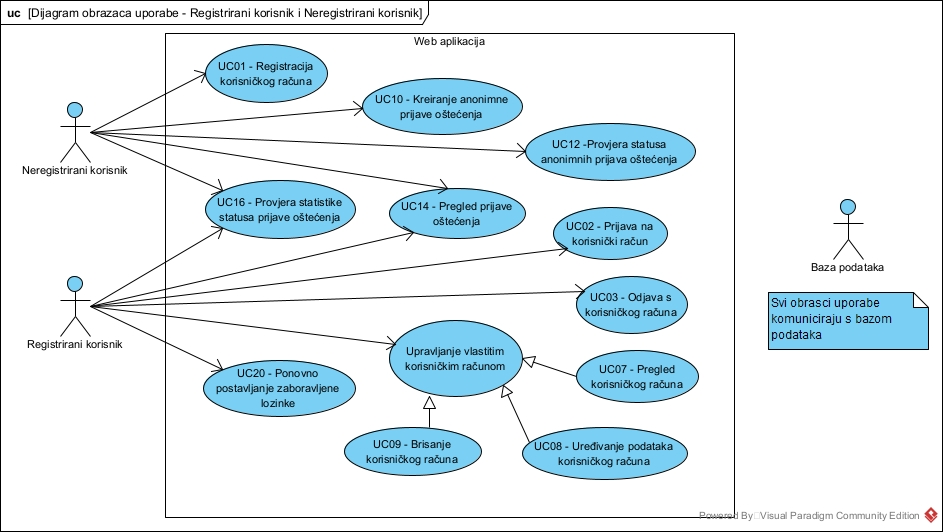
\includegraphics[scale=0.5]{slike/UC-registrirani-neregistrirani} %veličina slike u odnosu na originalnu datoteku i pozicija slike
	\centering
	\caption{Dijagram obrasca uporabe, funkcionalnost registriranog i neregistriranog korisnika}
	\label{fig:DijagramObrascaUporabeRegistriranNeregistriranKorisnik}
\end{figure}

\begin{figure}[H]
	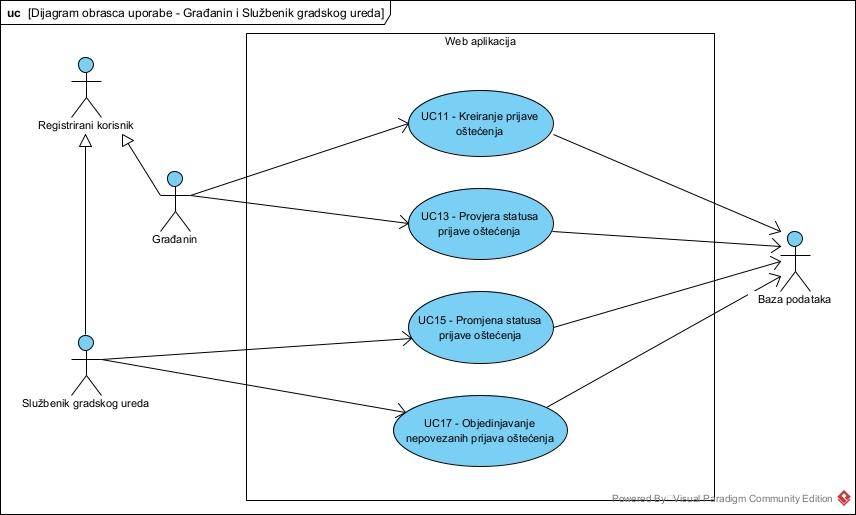
\includegraphics[scale=0.5]{slike/UC-gradanin-sluzbenik} %veličina slike u odnosu na originalnu datoteku i pozicija slike
	\centering
	\caption{Dijagram obrasca uporabe, funkcionalnost građanina i službenika gradskog ureda}
	\label{fig:DijagramObrascaUporabeGradaninSluzbenik}
\end{figure}

\begin{figure}[H]
	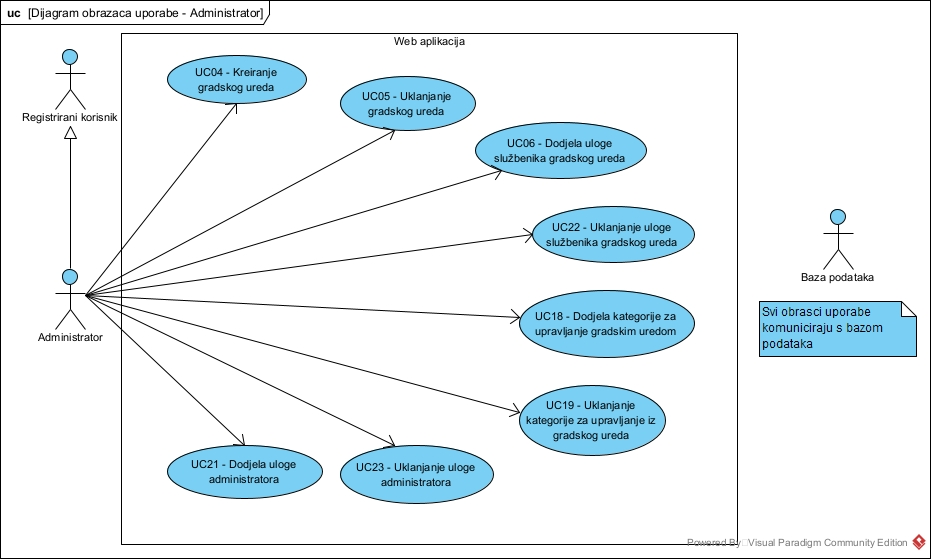
\includegraphics[scale=0.5]{slike/UC-administrator} %veličina slike u odnosu na originalnu datoteku i pozicija slike
	\centering
	\caption{Dijagram obrasca uporabe, funkcionalnost administratora}
	\label{fig:DijagramObrascaUporabeAdministrator}
\end{figure}

\eject

\subsection{Sekvencijski dijagrami}

\noindent \textbf{Obrazac uporabe UC11 - Kreiranje prijave oštećenja}

Registrirani korisnik šalje zahtjev za prikaz opcije kreiranja prijave oštećenja. Poslužitelj prikazuje stranica za kreiranje 
prijave oštećenja na kojoj korisnik unosi podatke o oštećenju. Postoje obvezni i neobvezni podaci. Dok korisnik ne unese sve 
obvezne podatke ne prikazuje se opcija za potvrdu unosa podataka. Kada unese sve obvezne podatke prikaže se opcija za potvrđivanja 
unosa podataka. Korisnik odlučuje hoće li unijeti neobvezne podatke poput fotografije oštećenja. Potvrđeni podaci spremaju se u 
bazu podataka. Ukoliko su podaci ispravni, poslužitelj prikazuje prikaz uspješnog kreiranja prijave oštećenja, a ukoliko nisu, 
poslužitelj prikazuje prikaz neuspješnog kreiranje prijave oštećenja s obrazloženjem razloga.

\begin{figure}[H]
	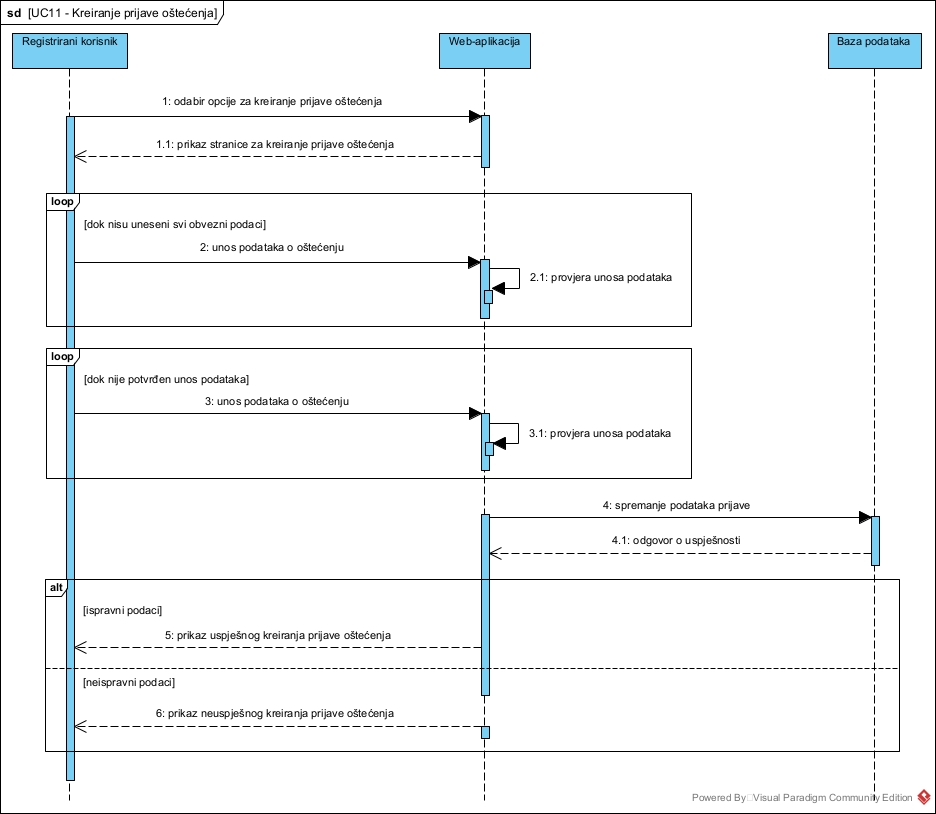
\includegraphics[scale=0.5]{slike/UC11_sekvencijski.jpg} %veličina slike u odnosu na originalnu datoteku i pozicija slike
	\centering
	\caption{Sekvencijski dijagram za UC11}
	\label{fig:SekvencijskiDijagramKreiranjePrijaveOštećenja}
\end{figure}

\noindent \textbf{Obrazac uporabe UC12 - Provjera statusa anonimne prijave oštećenja}

Neregistrirani korisnik šalje zahtjev za prikaz opcije za provjeru statusa anonimne prijave oštećenja. Poslužitelj prikazuje stranicu
za pregled statusa anonimne prijave oštećenja. Korisnik unosi jedinstveni broj prijave. Poslužitelj provjerava postoji li prijava oštećenja
s tim jedinstvenim brojem u bazi podataka. Ukoliko postoji, poslužitelj prikazuje podatke o oštećenju, a ukoliko ne postoji, poslužitelj prikazuje
poruku o neuspješnom unosu jedinstvenog broja prijave.


\begin{figure}[H]
	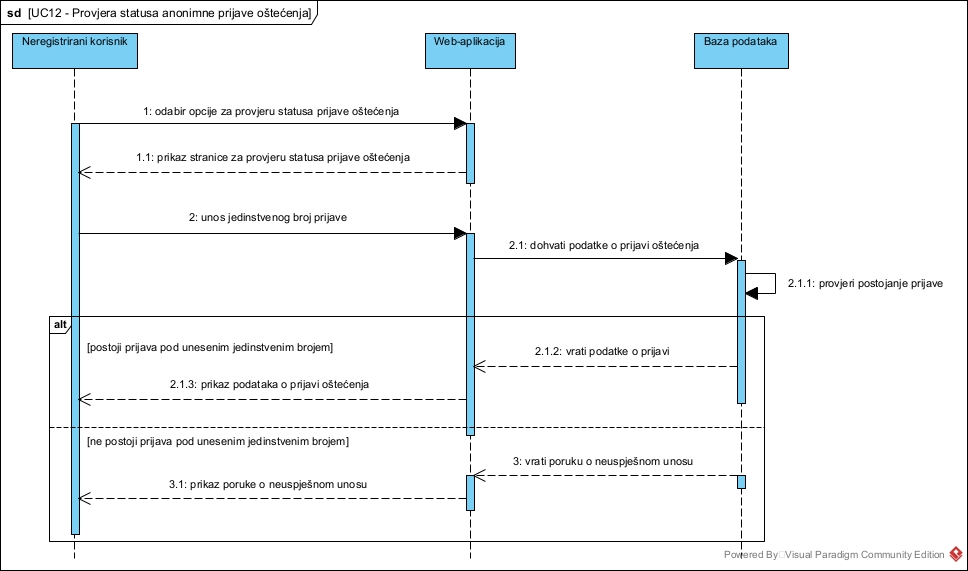
\includegraphics[scale=0.5]{slike/UC12_sekvencijski.jpg} %veličina slike u odnosu na originalnu datoteku i pozicija slike
	\centering
	\caption{Sekvencijski dijagram za UC12}
	\label{fig:SekvencijskiDijagramProvjeraStatusaAnonimnePrijaveOštećenja}
\end{figure}

\noindent \textbf{Obrazac uporabe UC15 - Promjena statusa prijave oštećenja}

Službenik gradskog ureda šalje zahtjev za prikaz popisa prijavljenih oštećenja. Poslužitelj dohvaća popis prijavljenih oštećenja iz baze 
podataka te ih prikazuje službeniku. Službenik odabire prijavu oštećenja te time šalje zahtjev za prikaz podataka o toj prijavi oštećenja. 
Poslužitelj dohvaća podatke o prijavi oštećenja te ih prikazuje službeniku. Službenik šalje zahtjev za prikaz opcije za promjenu statusa prijave
oštećenja. Poslužitelj prikazuje opciju za promjenu statusa prijave oštećenja s navedenim mogućim opcijama stanja prijave oštećenja. Službenik
odabire novi status prijave oštećenja te šalje zahtjev za promjenu statusa poslužitelju. Poslužitelj ažurira status prijave oštećenja u bazi
podataka. Poslužitelj prikazuje službeniku potvrdu o uspješnosti promjena statusa prijave oštećenja.

\begin{figure}[H]
	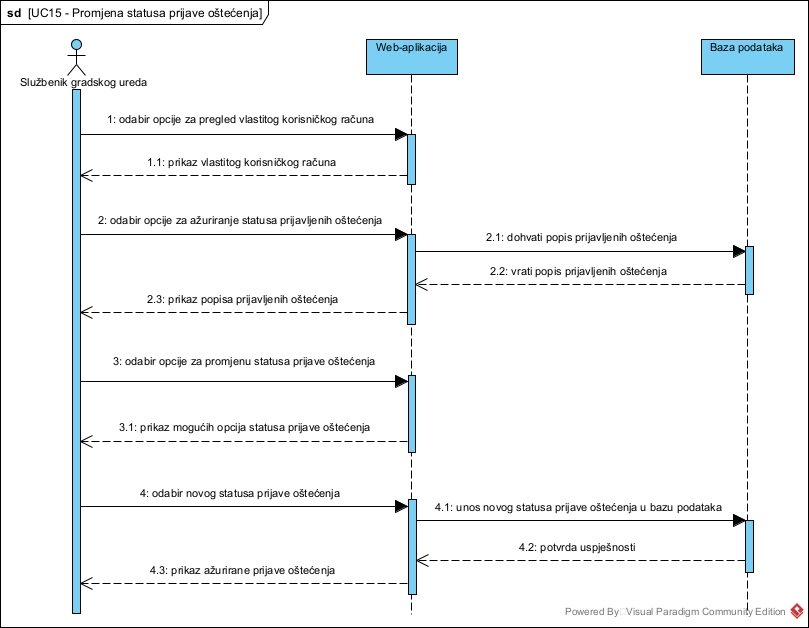
\includegraphics[scale=0.5]{slike/UC15_sekvencijski.jpg} %veličina slike u odnosu na originalnu datoteku i pozicija slike
	\centering
	\caption{Sekvencijski dijagram za UC15}
	\label{fig:SekvencijskiDijagramPromjenaStatusaPrijaveOštećenja}
\end{figure}

\noindent \textbf{Obrazac uporabe UC17 - Objedinjavanje nepovezanih prijava oštećenja}

Službenik gradskog ureda šalje zahtjev za prikaz popisa prijavljenih oštećenja. Poslužitelj dohvaća popis prijavljenih oštećenja iz baze 
podataka te ih prikazuje službeniku. Službenik odabire opciju za objedinjavanje prijava oštećenja. Poslužitelj prikazuje oznake za označavanje
prijava oštećenja. Službenik odabire prijave oštećenja. Službenik potvrđuje odabir prijava oštećenja za objedinjavanje. Poslužitelj unosi
podatke o objedinjenim prijavama oštećenja u bazu podataka. Događa se referenciranje objedinjene prijave oštećenja na postojećih prijava 
oštećenja. Po završetku, poslužitelj prikazuje službeniku gradskog ureda podatke objedinjene prijave oštećenja. 


\begin{figure}[H]
	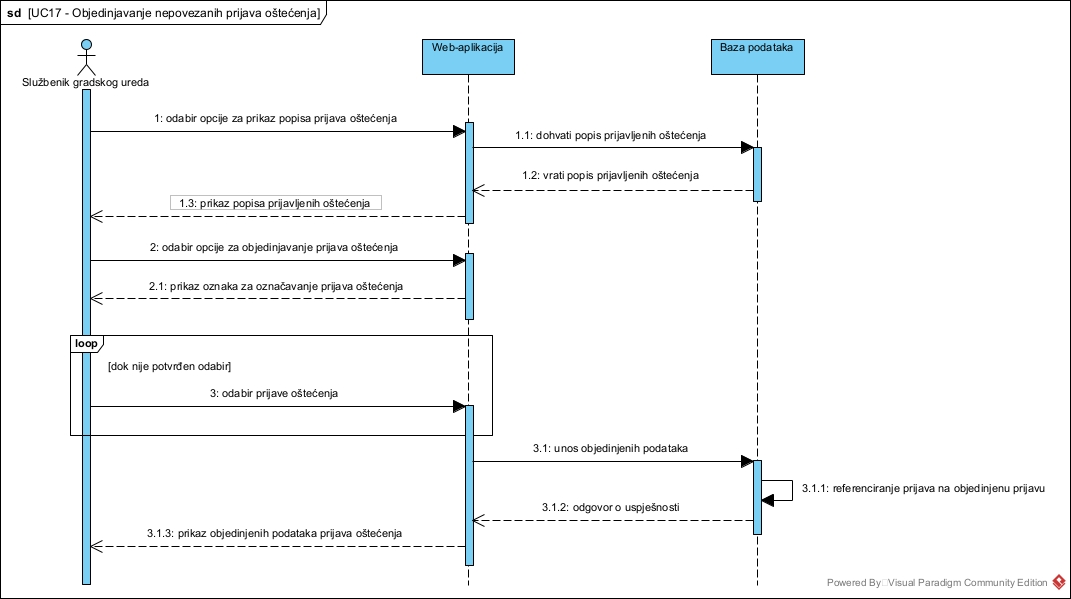
\includegraphics[scale=0.5]{slike/UC17_sekvencijski.jpg} %veličina slike u odnosu na originalnu datoteku i pozicija slike
	\centering
	\caption{Sekvencijski dijagram za UC17}
	\label{fig:SekvencijskiDijagramObjedinjavanjeNepovezanihPrijavaOštećenja}
\end{figure}

\eject

\section{Ostali zahtjevi}

\begin{packed_enum}
	\item Sustav treba podržavati rad više korisnika u stvarnom vremenu
	\item Sustav treba ispravno funkcionirati na svim web preglednicima
	\item Sustav treba biti izveden kao web aplikacija prilagođena mobilnom uređaju i tablet računalu
	\item Korisničko sučelje i sustav podržavaju hrvatsku abecedu (dijakritičke znakove) pri unosu i prikazu tekstualnog sadržaja
	\item Sustav koristi hrvatski jezik i srednjoeuropsko standardno vrijeme, GMT+1
	\item Korisničko sučelje treba biti jednostavno za korištenje bez opširnih uputa
	\item Neispravno korištenje korisničkog sučelja ne smije narušiti funkcionalnost i rad sustava 
	\item Sustav ne smije omogućiti registraciju korisnika i promjenu lozinke dok nije unesena dovoljno jaka lozinka duljine od barem 8 znakove te barem jedno malo slovo, veliko slovo, znamenku i specijalni znak
	\item Sustav sprema lozinku u sigurnom obliku različitom od običnog tekstualnog formata, koristeći bcrypt hash
	\item Sustavu se pristupa s javne mreže pomoću HTTPS
	\item Pristupanje bazi podataka ne smije trajati duže od nekoliko sekundi
	\item Buduće nadogradnje sustava ne smiju narušiti postojeće funkcionalnosti sustava
\end{packed_enum}

